\scanpage{142}
\uline{Le foncteur} $\Phi$ \uline{est pleinement fidèle} (On est ramené au cas de la base $\eta=\operatorname{Spec}K$).

L'image essentielle est \deleted{\uline{\unsure{contenue}} dans} formée des motifs $(M,\{E_\ell\},\{u_\ell\})$ tels que \deleted{les $E_\ell$} leur quotient modulo torsion soit associé à un \uline{schéma} \uline{abélien} sur $S$.

Il \uline{faut} \uline{\unsure{pour|voir}} cela que $M$ soit effectif de poids $1$, i.e. soit défini par un schéma abélien \inserted{$A_K$} sur $K$. \deleted{\unsure{Il} \unsure{Mais}}

La question si cette \unsure{question|condition} est suffisante revient à celle-ci : Soit $A$ un schéma abélien sur $K$, \deleted{de} tel que $\forall\,\ell$, \deleted{les} $T_\ell(A)$ soit non ramifié sur $S_\ell$, alors $A$ a bonne réduction sur $S$. Cela marche si $S$ est de dim $1$\inserted{ (critère de \inserted{\unsure{Néron}-}Ogg-\unsure{Chafarevitch|Chafarévitch|Chafarevich})}, \uline{ou} si $S$ de car. nulle (critère de \unsure{mézigues}), mais peut-être pas en général (p.ex. anneau local régulier de dim $2$ d'inégales caractéristiques). Pour faire un contre-exemple, il suffirait d'avoir un exemple d'un schéma abélien $A$ sur $S$, et d'un ss-groupe fini de $A_K$ qui ne se prolonge pas en un ss-groupe \uline{fini} et \uline{plat} de $A$. S'il y avait un tel exemple, il y en aurait aussi avec un ordre premier.....

\margin{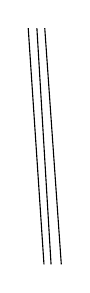
\begin{tikzpicture}[x=1mm,y=1mm]\draw (0,30)--(2,0) (1.1,30)--(2.9,0) (2.1,30)--(4.2,0);\end{tikzpicture}}
\uline{Pb} Avec la définition adoptée de motif lisse (en termes de celle de isomotif lisse, comme un isomotif \uline{sur} $K$ avec simplement une propriété \inserted{``galoisienne''} de non ramification pour les $T_\ell$) il n'est pas du tout \unsure{claire|clair} comment définir l'image inverse d'un motif (resp. d'un isomotif) par $S'\unsure{\mathord{-}|\to}S$, p.ex. des fibres en les $s\in S$. Cette difficulté \deleted{\unsure{se pose}}\inserted{concerne} en fait les isomotifs, et vaut déjà pour ceux qui sont effectifs de poids $1$.
% archive sheet number: 141
